\documentclass[apj, revtex4]{emulateapj}

%%%%% AUTHORS - PLACE YOUR OWN PACKAGES HERE %%%%%
%\usepackage{amsmath}	% Advanced maths commands
%\usepackage{amssymb}	% Extra maths symbols
%\usepackage{mathrsfs}	% Extra extra math symbols

\usepackage{epsf}
\usepackage{color}
\usepackage{amsmath}
\usepackage{graphicx}
\usepackage[colorlinks,urlcolor=magenta,citecolor=blue,linkcolor=blue]{hyperref}
\usepackage{threeparttable}
\usepackage{multirow}
\usepackage{natbib}
\usepackage{etoolbox}
\usepackage{longtable}

\bibliographystyle{apj}
\citestyle{aa}

%%%%% AUTHORS - PLACE YOUR OWN COMMANDS HERE %%%%%
%%% Fields %%%
\newcommand{\hdf}{HDF-N}
\newcommand{\hdfn}{HDF-N}
\newcommand{\hdfs}{HDF-S}
\newcommand{\cdfs}{CDF-S}

%%% Telescopes %%%
\newcommand{\hst}{\textit{HST}}
\newcommand{\iras}{\textit{IRAS}}
\newcommand{\iso}{\textit{ISO}}
\newcommand{\spitzer}{\textit{Spitzer}}
\newcommand{\sirtf}{\textit{Spitzer}}
\newcommand{\chandra}{\textit{Chandra}}
\newcommand{\planck}{\textit{Planck}}

%%% Filters %%%
\newcommand{\wfu}{\hbox{$\mathrm{U}_{300}$}}
\newcommand{\wfb}{\hbox{$\mathrm{B}_{450}$}}
\newcommand{\wfv}{\hbox{$\mathrm{V}_{606}$}}
\newcommand{\wfi}{\hbox{$\mathrm{I}_{814}$}}
\newcommand{\acsb}{\hbox{$\mathrm{B}_{435}$}}
\newcommand{\acsv}{\hbox{$\mathrm{V}_{606}$}}
\newcommand{\acsi}{\hbox{$i_{775}$}}
\newcommand{\acsz}{\hbox{$z_{850}$}}
\newcommand{\nicj}{\hbox{$\mathrm{J}_{110}$}}
\newcommand{\nich}{\hbox{$\mathrm{H}_{160}$}}
\newcommand{\wfcy}{\hbox{$\mathrm{Y}_{105}$}}
\newcommand{\wfcj}{\hbox{$\mathrm{J}_{125}$}}
%\newcommand{\wfcj}{\hbox{$J_{110}$}}
\newcommand{\wfch}{\hbox{$\mathrm{H}_{160}$}}
\newcommand{\sdssu}{\hbox{$u$}}
\newcommand{\sdssg}{\hbox{$g$}}
\newcommand{\sdssr}{\hbox{$r$}}
\newcommand{\sdssi}{\hbox{$i$}}
\newcommand{\sdssz}{\hbox{$z$}}
\newcommand{\mone}{\hbox{$[3.6]$}}
\newcommand{\mtwo}{\hbox{$[4.5]$}}
\newcommand{\mthree}{\hbox{$[5.8]$}}
\newcommand{\mfour}{\hbox{$[8.0]$}}
%\newcommand{\mone}{\hbox{$[3.6\mu\mathrm{m}]$}}
%\newcommand{\mtwo}{\hbox{$[4.5\mu\mathrm{m}]$}}
%\newcommand{\mthree}{\hbox{$[5.8\mu\mathrm{m}]$}}
%\newcommand{\mfour}{\hbox{$[8.0\mu\mathrm{m}]$}}

%%% Astronomy Abreviations %%%
\newcommand{\mstar}{\hbox{M$_{\star}$}}
\newcommand{\lstar}{\hbox{L$_{\star}$}}
\newcommand{\Msol}{\hbox{$\mathrm{M}_\odot$}}
\newcommand{\msol}{\hbox{$\mathrm{M}_\odot$}}
\newcommand{\Zsol}{\hbox{$Z_\odot$}}
\newcommand{\zsol}{\hbox{$Z_\odot$}}
\newcommand{\Lsol}{\hbox{$L_\odot$}}
\newcommand{\lsol}{\hbox{$L_\odot$}}
\newcommand{\lir}{\hbox{$L_{\mathrm{IR}}$}}
\newcommand{\zph}{\hbox{$z_\mathrm{ph}$}}
\newcommand{\zphot}{\hbox{$z_\mathrm{ph}$}}
\newcommand{\lbol}{\hbox{$L_\mathrm{bol}$}}
\newcommand{\snr}{\hbox{$\mathrm{S/N}$}}
\newcommand{\reff}{\hbox{$r_\mathrm{eff}$}}
\newcommand{\ks}{\hbox{$K_s$}}
\newcommand{\AAA}{\hbox{\AA}}

%%% Spectrum Lines %%%
\newcommand{\lya}{ Ly$\alpha \;$}
\newcommand{\lyb}{Lyman~$\beta$}
\newcommand{\hb}{\hbox{H$\beta$}}
\newcommand{\ha}{\hbox{H$\alpha$}}
\newcommand{\paa}{\hbox{Pa$\alpha$}}

%%% Units %%%
\newcommand{\kms}{\hbox{km~s$^{-1}$}}
\newcommand{\cms}{\hbox{cm~s$^{-1}$}}
\newcommand{\ergscm}{\hbox{erg~s$^{-1}$~cm$^{-2}$}}
\newcommand{\cnts}{\hbox{cnt~s$^{-1}$}}
\newcommand{\uJy}{\hbox{$\mu$Jy}}
\newcommand{\ujy}{\hbox{$\mu$Jy}}
\newcommand{\degree}{\hbox{$^\circ$}}
\newcommand{\degsq}{\hbox{degree$^2$}}
\newcommand{\arcminsq}{\hbox{arcmin$^2$}}
\newcommand{\um}{\hbox{$\mu$m}}

%%% per Units %%%
\newcommand{\perarcminsq}{\hbox{arcmin$^{-2}$}}
\newcommand{\perdegsq}{\hbox{degree$^{-2}$}}
\newcommand{\permpc}{\hbox{Mpc$^{-1}$}}
\newcommand{\permpcsq}{\hbox{Mpc$^{-2}$}}
\newcommand{\permpccu}{\hbox{Mpc$^{-3}$}}
\newcommand{\percmsq}{\hbox{cm$^{-2}$}}
\newcommand{\percmcu}{\hbox{cm$^{-3}$}}
\newcommand{\perpixel}{\hbox{pixel$^{-1}$}}

%%% Math %%%
\newcommand{\lsim}{\lesssim}
\newcommand{\gsim}{\gtrsim}
\newcommand{\mathS}{\hbox{$\mathcal{S}$}}
\newcommand{\mathR}{\hbox{$\mathcal{R}$}}
\newcommand{\mathM}{\hbox{$\mathcal{M}$}}
\newcommand{\mcal}{\hbox{$\mathcal{M}$}}
\newcommand{\rcal}{\hbox{$\mathcal{R}$}}
\newcommand{\scal}{\hbox{$\mathcal{S}$}}
\newcommand{\infinity}{\hbox{$\infty$}}
\newcommand{\err}[2]{$^{+#2}_{-#1}$}

%%% General %%%
\newcommand{\etal}{et al.}
\newcommand{\eg}{e.g.}
\newcommand{\ie}{i.e.}
\newcommand{\cf}{cf.}
% \newcommand{\ion}[2]{\hbox{#1$\;${\small\rm{#2}}}}
\newcommand{\mybullet}{\noindent$\bullet$}
\newcommand{\uit}{\textit{UIT}}
\newcommand{\nd}{...}
%\newcommand{\cmodel}{\hbox{\tt cmodel}}
%\newcommand{\bs}{\hbox{$\!\!\!\!$}}
\newcommand{\todo}[1]{{\tt #1}}
\newcommand{\citeeg}[1]{(\eg, \citealt{#1})}
\newcommand{\ignore}[1]{}

%%% Extra %%%
% \newcommand{\farcm}{\mbox{\ensuremath{.\mkern-4mu^\prime}}}    % fractional arcminute symbol: 0.'0
% \newcommand{\farcs}{\mbox{\ensuremath{.\!\!^{\prime\prime}}}}  % fractional arcsecond symbol: 0.''0
% \newcommand{\fdg}{\mbox{\ensuremath{.\!\!^\circ}}}             % fractional degree symbol:    0.°0
%\newcommand{\arcdeg}{\ensuremath{^{\circ}}}%                    % degree symbol:  °
% \newcommand{\sun}{\ensuremath{\odot}}%                         % sun symbol
% \newcommand{\apj}{ApJ}%                                        % Journal abbreviations
% \newcommand{\apjs}{ApJS}
% \newcommand{\apjl}{ApJL}
% \newcommand{\aap}{A{\&}A}
% \newcommand{\aaps}{A{\&}AS}
% \newcommand{\mnras}{MNRAS}
% \newcommand{\aj}{AJ}
% \newcommand{\araa}{ARAA}
% \newcommand{\pasp}{PASP}
\newcommand{\Teff}{\ensuremath{T_{\mathrm{eff}}}}%               % T_eff
\newcommand{\logg}{\ensuremath{\log g}}%                         % log g
%\newcommand{\bv}{\ensuremath{B\!-\!V}}%                         % B-V
%\newcommand{\ub}{\ensuremath{U\!-\!B}}%                         % U-B
%\newcommand{\vr}{\ensuremath{V\!-\!R}}%                         % V-R
%\newcommand{\ur}{\ensuremath{U\!-\!R}}%                         % U-R
%\newcommand\ion[2]{#1$\;${\scshape{#2}}}%                       % ion, i.e., CII = \ion{C}{ii}


\newcommand{\editorial}[1]{\textcolor{red}{#1}}
\newcommand{\multic}[2]{\multicolumn{#1}{c}{#2}}
\newcommand{\rottext}[2]{\multirow{#1}{*}{\rotatebox[origin=c]{90}{#2}}}

\makeatletter
% Patch case where name and year are separated by aysep
\patchcmd{\NAT@citex}
{\@citea\NAT@hyper@{%
		\NAT@nmfmt{\NAT@nm}%
		\hyper@natlinkbreak{\NAT@aysep\NAT@spacechar}{\@citeb\@extra@b@citeb}%
		\NAT@date}}
{\@citea\NAT@nmfmt{\NAT@nm}%
	\NAT@aysep\NAT@spacechar\NAT@hyper@{\NAT@date}}{}{}

% Patch case where name and year are separated by opening bracket
\patchcmd{\NAT@citex}
{\@citea\NAT@hyper@{%
		\NAT@nmfmt{\NAT@nm}%
		\hyper@natlinkbreak{\NAT@spacechar\NAT@@open\if*#1*\else#1\NAT@spacechar\fi}%
		{\@citeb\@extra@b@citeb}%
		\NAT@date}}
{\@citea\NAT@nmfmt{\NAT@nm}%
	\NAT@spacechar\NAT@@open\if*#1*\else#1\NAT@spacechar\fi\NAT@hyper@{\NAT@date}}

%%%%%%%%%%%%%%%%%%% TITLE PAGE %%%%%%%%%%%%%%%%%%%
 %-----------------------------------------------------------------------------------------

\shorttitle{}
\shortauthors{BOADA ET AL.}

\slugcomment{\it Draft Version \today}
%\slugcomment{\it Submitted for publication in the Astrophysical Journal}
%\slugcomment{Accepted for Publication in the Astrophysical Journal}

\begin{document}

\title{Planck Cluster Paper}

\author{\sc SB\altaffilmark{1}, JPH\altaffilmark{1}, FM, PD\altaffilmark{1}}

\altaffiltext{1}{Rutgers;boada@physics.rutgers.edu}


\begin{abstract}
	\noindent We propose to continue our program of optical imaging to unveil all of the most massive clusters in
	the observable Universe. We start from the all-sky \textit{Planck} Sunyaev-Zel’dovich (SZ) catalogs, which contain several hundred high significance (signal-to-noise ratio, SNR $> 5$) unconfirmed cluster candidates. Since SZ selection favors high mass clusters and the \textit{Planck} confirmation process favored	low redshift systems, the highest significance unconfirmed candidates are, therefore, likely massive clusters ($M_{500} > 5 ×\times 10^{14}$ \Msol) at relatively high redshift ($z > 0.5$). Our proposed observations,	using MOSAIC-3 on Mayall, are designed to confirm the presence of a brightest cluster galaxy (to $z \sim 1$) and red sequence of accompanying cluster members (to $z \sim 0.7$). Preliminary results from our observations over the past two years have validated our approach by the detection of optical clusters in a number of \textit{Planck} candidates, including the discovery of rich systems at $z = 0.553$ and $z = 0.830$ that rival the most massive clusters known. The proposed observations represent the first step required to provide a complete all-sky census throughout the observable Universe of the most massive, high redshift clusters. Their expected high redshift and high mass make the unconfirmed \textit{Planck} clusters, arguably, the most important available sample for probing deviations from $\Lambda$CDM and defining the high-mass end of the cluster mass function.
\end{abstract}

\section{Introduction}
\editorial{this section has not been edited and is just a bunch of stuff copy and pasted. I did update some of the references.}

Massive clusters of galaxies are the extraordinary objects which hold important clues to the evolution of structure in the universe. The widely accepted $\Lambda$CDM model of cosmology makes specific predictions about the mass distribution of galaxy clusters in the universe. The number of galaxy clusters, especially at high redshifts, can help constrain structure formation models (\eg, Mortonson et al. 2011; Harrison \& Coles 2012; Harrison \& Hotchkiss 2012; Waizmann et al. 2012; Zitrin et al. 2009). Galaxy clusters also harbor a significant fraction of the visible baryons in the Universe, in the form of a hot intracluster medium that leaves an imprint on the Cosmic Microwave Background (CMB) though the Sunyaev-Zel'dovich effect (SZ; \citealt{Sunyaev1972} effect.

Using the SZ effect to discover clusters of galaxies has the distinct advantage that the surface brightness of the SZ effect does not dim with increasing redshift. This allows homogeneous samples of massive clusters to be detected out to arbitrary distances. Ground based, large area-sky surveys such as those with the Atacama Cosmology Telescope (ACT; \citealt{Swetz2011}) and the South Pole Telescope (SPT; \citealt{Carlstrom2011} have produced catalogs of hundreds of massive clusters below $z \sim 1.4$ \citeeg{Hasselfield2013a, Reichardt2013a}. Now, \textit{Planck} \citep{Tauber2010, PlanckCollaboration2011} has released an all-sky SZ sample (PSZ; \citealt{PlanckCollaboration2014, PlanckCollaboration2015}) that contains 861 confirmed clusters (of which most [683] were known previously) and another 366 unconfirmed cluster candidates.

Clusters were initially confirmed by cross correlating with previous catalogs (see Section 4; \citealt{PlanckCollaboration2014}). More recently, dedicated follow up of still-unconfirmed clusters has begun in earnest \citeeg{Liu2015a, PlanckCollaboration2015, PlanckCollaboration2016a, Burenin2017, Barrena2018, Amodeo2018, Streblyanska2018}.

This paper is organized as follows: sections \ref{sec:design} through \ref{sec:analysis} describe the design, observations, data reduction and calibration, and creation of derived data products. In Section~\ref{sec:results}, we present the main results of our observations, and discuss the results in Section~\ref{sec:discussion}. In Section~\ref{sec:summary}, we summarize the key results and conclude.

Unless otherwise noted, throughout this paper, we use a concordance cosmological model ($\Omega_\Lambda = 0.7$, $\Omega_m = 0.3$, and $H_0= 70$ \kms \mpc), assume a Chabrier initial mass function \citep{Chabrier2003}, and use AB magnitudes \citep{Oke1974}.

\section{Design}\label{sec:design}
Among the recently released, second, all-sky PSZ catalog\footnote{\hbox{\url{http://szcluster-db.ias.u-psud.fr/sitools/client-user/SZCLUSTER_DATABASE/project-index.html}}} (hereafter PSZ2; \citealt{PlanckCollaboration2015}) there are 450 unconfirmed SZ detections with S/N $> 4.5$. The vast majority of these must lie at high-z because the \textit{Planck} confirmation process \citep{PlanckCollaboration2014} mostly relied on existing catalogs with a preference for low-z clusters. Furthermore, the confirmed sample has a small fraction (3\%) of $z > 0.6$ clusters compared to that expected ($\sim20$\%) based on the theoretical halo mass function \citeeg{Jenkins2001, Tinker2008}. If other clusters like ``El Gordo'' exist, they are hiding as high-significance candidates within the objects in this catalog. The design of the observations is to use optical imaging to confirm the SZ detections as real clusters and provide photometric redshifts using the multi-color information.

We design the observations based on the previous success with the ACT cluster confirmation process using 4-m class telescopes. Our strategy is to use the Kitt Peak National Observatory (KPNO) Mayall-4m telescope imaging as the first and fundamental step to confirm the highest significance detections in the PSZ2 catalog that are visible across the entire northern sky. Following closely the procedure used for ACT follow-up \editorial{citation?}, targets are prioritized by SZ signal-to-noise (S/N). We choose to initially report on targets with PSZ2 S/N $>5$ as the statistical reliability of PSZ2 cluster candidates is quite high: according to the \textit{Planck} team $\sim90$\% of candidates at S/N $>5$ turn out to be ``real'' clusters (\editorial{citation? maybe show the figure from the proposal}).

Optical imaging will be sufficient to confirm nearly all of the candidates, but for the highest redshift ones, NIR data will be necessary. Again following the procedure for ACT cluster follow-up: those candidates with some evidence for a high-z brightest cluster galaxy (BCG; \editorial{note that we can detect BCGs to $z \sim 1.5$}) will be targeted with NIR observations to confirm the presence of a BCG and detect the red sequence of cluster members. Observational priority again is given to higher S/N candidates.

%We led the ACT cluster confirmation process using 4-m class telescopes; now we propose to use our well-established expertise to identify \textit{Planck} clusters. The recent SZ cluster samples have opened a new window into extreme systems, the most massive clusters at high redshift \citep{Foley2011, Menanteau2012}, prompting studies that match their observed numbers with the abundance predictions of $\Lambda$CDM cosmology (Hoyle et al. 2011, Mortonson et al. 2011, Waizmann et al. 2012). There are few, if any, clusters at high redshift ($z > 0.8$) and high mass ($M_{200} > 10^{15}$ \Msol\ ) in the cosmological simulations (see \citealt{Tinker2008}), so the halo mass function at high-z and high-M is essentially unconstrained. Thus, with the proposed observations we will determine the abundance of massive clusters at high redshift making a direct observational measurement of the high-z, high-M end of the halo mass function. For example, one of the most impressive results of the ACT SZ survey is our discovery of the high redshift ($z = 0.87$), extreme cluster ``El Gordo'' (ACT-CL J0102-4915), the most significant SZ detection of the whole survey (and also of the SPT survey). Our recent HST weak-lensing analysis has provided an independent mass estimation $M_{200a} = (3.1 \pm 0.7)\times 10^{15}$ \Msol\ (Jee et al. 2013) that confirms our earlier mass estimates for the cluster \citep{Menanteau2012}. Based on its estimated mass alone, ``El Gordo'' is a very rare system within the ACT+SPT (2800 sq. deg.) survey area, but is still consistent with the expectations of $\Lambda$CDM. We are now at a unique moment in cluster science where we can discover all massive clusters in the observable universe. This census will measure the high-mass, high-redshift cluster mass function, and determine the extent of deviations from the theoretical halo mass function \citep{Jenkins2001, Tinker2008}.

%Assuming WMAP7 cosmology \citep{Komatsu2011} with the \cite{Tinker2008} halo mass function, there should be only $\sim4$ clusters as massive as “El Gordo” ($\leq 2 \times 10^{15}$ \Msol) at $z > 0.6$ in the full area covered by the \textit{Planck} PSZ catalog (83.7\% of the sky). Although \textit{Planck}’s larger beam size (compared to both ACT and SPT) makes it more sensitive to clusters at lower redshifts (due to their larger projected area on the sky), among the 861 confirmed clusters in the recently released all-sky \textit{Planck} SZ catalog are the two highest significance high-redshift SZ detections from ACT (as well as several other ACT and SPT clusters). This confirms the ability of \textit{Planck} to unambiguously detect the most massive clusters at high redshift. In fact \textit{Planck} reports ``El Gordo'' ($z = 0.87$) and ACT-CL J2327.4−0204 ($z = 0.701$) at S/N values of 8.0 and 6.3, respectively. And as Figure 2 (right panel) shows, these are the two most massive \textit{Planck} clusters in the confirmed sample at high redshift. For the new clusters we confirm, our experimental design allows us to estimate photometric redshifts, which will be sufficiently accurate for a meaningful estimate of the cluster’s mass from the \textit{Planck} SZ signal.

% For semester 2014A alone, this corresponds to a sky area of $\sim20,000$ sq. deg., more than 6 times the area of the current combined ACT+SPT surveys. Following closely the procedure we used for ACT follow-up, we prioritize the target selection by SZ signal-to-noise (S/N). For this initial investigation we will target the $\sim60$ cluster candidates (visible in 2014A) from the PSZ catalog with S/N$>5$. For this sample the statistical reliability of PSZ cluster candidates is quite high: according to the \textit{Planck} team $\sim90$\% of candidates at S/N$>5$ turn out to be ``real'' clusters (see Fig. 2, left panel). Given this purity value, the proposed observations, utilizing telescopes in both hemispheres, will enable the confirmation of $\approx 50 − 60$ massive clusters at high redshift in semester 2014A alone. We will propose to observe the remaining S/N$>5$ PSZ candidates during semester 2014B.

\subsection{Observations}\label{sec: observations}
All observations were conducted with the KPNO Mayall telescope. The optical observations were made with the MOSAIC camera mounted at the prime focus. Two detector packages were used for the observations. The earlier MOSAIC1.1 instrument consisted of eight $2048\times4096$ SITe CCDs, arranged $2\times4$, separated by a $∼\sim50$ pixels gap with a pixel scale of $0\farcs26$ pixel$^{-1}$. MOSAIC1.1 was replaced with Mosaic3, in \editorial{year?},  and consists of four new 4k$\times$4k, 15 micron pixel, 500-micron thick LBNL deep-depletion CCDs. Because the only change from MOSAIC1.1 to MOSAIC3 are the CCDs and controllers both versions have a $36' \times 36'$ field-of-view.

\editorial{need to talk about the dithering}

The optical observing strategy consists of targeted $griz$ observations of individual candidates with exposure times of 350 s, 350 s, 1100 s and 1100 s (assuming dark conditions) to provide $5\sigma$ detections limits of \editorial{$g=??$}, $r = 24.5$, $i = 24.5$, $z = 24.2$ ensuring the unambiguous detection of the faint (i.e., 0.4L$_∗\star$ ) galaxies in the red cluster sequence up to $z \sim 1.0$ \editorial{(citation?)} and of brightest cluster galaxies (BCGs) to higher redshifts. The choice of filters in our program is driven by the need to segregate early-type galaxies in the cluster through their colors (or photometric redshifts) by sampling blue-ward and red-ward of the 4000\AA\ break. \editorial{Our depths are quite a bit different that the designed depths. Should we mention that here, or wait till later on when we are discussing how we actually did?}

\begin{longtable*}{lcccccc}
	\caption[Basic properties of the galaxy cluster candidates targeted for observation.]{Basic properties of the galaxy clusters candidates targeted for observation with the MOSAIC and NEWFIRM instruments: Column 1: Cluster name; Column 2: The right ascension of the cluster; Column 3: The declination of the cluster; Column 4: the PSZ1 catalog S/N ratio; Column 5: the PSZ2 catalog S/N ratio; Column 6: The date of MOSAIC observations}\\
	\hline
	Cluster & RA (J2000) & DEC (J2000) & PSZ1 SNR & PSZ2 SNR & MOSAIC Obs. \\
	(1) & (2) & (3) & (4) & (5) & (6) \\
	\hline \hline
	\endfirsthead
	\multicolumn{4}{l}%
	{\tablename\ \thetable\ Continued} \\
	\hline
	Cluster & RA (J2000) & DEC (J2000) & PSZ1 SNR & PSZ2 SNR & MOSAIC Obs. \\
	(1) & (2) & (3) & (4) & (5) & (6) \\
	\hline \hline
	\endhead
PSZ1 G031.91+67.94 & 14:29:02 & +24:37:33.38 & 5.23 & nan & Feb, 2014\\
PSZ1 G055.83-41.64 & 21:57:14 & -2:31:51 & 5.72 & nan & Oct, 2014\\
PSZ1 G084.62-15.86 & 21:49:44 & +33:10:23.81 & 6.01 & nan & Oct, 2014\\
PSZ1 G096.44-10.40 & 22:19:35 & +44:31:05.27 & 6.55 & nan & Oct, 2014\\
PSZ1 G102.86-31.07 & 23:33:08 & +28:43:51.60 & 6.12 & nan & Oct, 2014\\
PSZ1 G102.97-04.77 & 22:34:47 & +52:43:13.90 & 5.64 & nan & Oct, 2014\\
PSZ1 G105.91-38.39 & 23:53:54 & +22:34:21.09 & 7.16 & nan & Oct, 2014\\
PSZ1 G108.90-52.04 & 0:16:38 & +09:52:49.98 & 6.89 & nan & Jun, 2017\\
PSZ1 G118.06+31.10 & 15:54:34 & +84:10:37.49 & 6.00 & nan & Feb, 2014\\
PSZ1 G127.55+20.84 & 3:10:51 & +82:25:43.91 & 5.91 & nan & Oct, 2014\\
PSZ1 G138.60-10.85 & 2:27:02 & +49:04:54.07 & 8.26 & nan & Oct, 2014\\
PSZ1 G142.17+37.28 & 9:18:56 & +70:52:01.14 & 5.79 & nan & Feb, 2014\\
PSZ1 G142.38+22.82 & 6:13:40 & +71:52:21.02 & 5.82 & nan & Feb, 2014\\
PSZ1 G146.00-49.42 & 1:51:35 & +10:44:02.79 & 6.62 & nan & Oct, 2014\\
PSZ1 G148.20+23.49 & 6:37:46 & +66:54:24.40 & 8.40 & nan & Feb, 2014\\
PSZ1 G153.41+36.58 & 8:42:40 & +62:34:31.61 & 6.85 & nan & Feb, 2014\\
PSZ1 G153.56+36.23 & 8:39:31 & +62:31:30.58 & 5.96 & nan & Feb, 2014\\
PSZ1 G162.30-26.92 & 3:24:26 & +24:00:44.46 & 6.56 & nan & Oct, 2014\\
PSZ1 G169.80+26.10 & 7:30:08 & +48:20:02.06 & 5.32 & nan & Oct, 2014\\
PSZ1 G183.26+12.25 & 6:42:56 & +31:49:07.58 & 5.43 & nan & Oct, 2014\\
PSZ1 G185.93-31.21 & 4:11:39 & +06:16:00.67 & 5.90 & nan & Jan, 2014\\
PSZ1 G206.45+13.89 & 7:29:59 & +11:56:22.64 & 5.90 & nan & Feb, 2014\\
PSZ1 G224.82+13.62 & 8:01:42 & -4:03:54 & 5.51 & nan & Jan, 2014\\
PSZ1 G249.01+73.75 & 11:56:46 & +16:55:43.68 & 7.14 & nan & Feb, 2014\\
PSZ1 G286.25+62.68 & 12:21:10 & +00:47:34.05 & 5.52 & nan & Feb, 2014\\
PSZ1 G341.69+50.66 & 14:25:20 & -4:59:54 & 5.48 & nan & Feb, 2014\\
PSZ2 G022.03+17.75 & 17:28:37 & -1:13:03 & 5.64 & 6.20 & Jun, 2017\\
PSZ2 G023.05+20.52 & 17:20:47 & +00:58:06.58 & nan & 5.57 & Jun, 2017\\
PSZ2 G024.46-18.08 & 19:42:23 & -15:26:09 & nan & 6.98 & Jun, 2017\\
PSZ2 G027.77+10.88 & 18:03:22 & +00:25:57.59 & nan & 6.42 & Jun, 2016\\
PSZ2 G028.15-08.62 & 19:13:41 & -8:08:26 & 5.07 & 7.67 & Jun, 2017\\
PSZ2 G029.66-47.63 & 21:45:44 & -21:46:49 & nan & 5.74 & Nov, 2016\\
PSZ2 G029.80-17.40 & 19:48:32 & -10:31:40 & 6.59 & 9.01 & Jun, 2016\\
PSZ2 G031.41-19.16 & 19:57:41 & -9:53:56 & 4.60 & 5.69 & Jun, 2017\\
PSZ2 G032.12-14.96 & 19:43:34 & -7:27:45 & 8.21 & 9.12 & Jun, 2017\\
PSZ2 G033.27-17.54 & 19:54:52 & -7:36:11 & 5.78 & 6.86 & Jun, 2017\\
PSZ2 G036.69-15.67 & 19:54:05 & -3:50:23 & nan & 5.69 & Jun, 2017\\
PSZ2 G043.44-41.27 & 21:36:44 & -10:17:48 & nan & 5.55 & Jun, 2017\\
PSZ2 G044.83+10.02 & 18:36:39 & +15:04:49.72 & 7.27 & 9.27 & Oct, 2015\\
PSZ2 G045.50-08.62 & 19:45:25 & +07:04:29.08 & 4.57 & 5.63 & Jun, 2017\\
PSZ2 G047.53+08.55 & 18:46:59 & +16:50:35.39 & 5.82 & 6.55 & Jun, 2016\\
PSZ2 G048.47+34.86 & 17:02:08 & +27:08:48.05 & nan & 5.74 & Jun, 2016\\
PSZ2 G065.35-08.01 & 20:26:04 & +24:08:06.72 & nan & 5.83 & Jun, 2016\\
PSZ2 G071.67-42.76 & 22:30:54 & +05:42:05.22 & 8.82 & 8.63 & Oct, 2014\\
PSZ2 G075.08+19.83 & 18:46:48 & +45:46:33.27 & nan & 5.74 & Jun, 2016\\
PSZ2 G089.06-11.79 & 21:52:53 & +39:03:52.50 & nan & 5.72 & Nov, 2016\\
PSZ2 G092.11-33.73 & 23:01:37 & +22:28:59.71 & nan & 5.81 & Nov, 2016\\
PSZ2 G092.46-35.22 & 23:05:50 & +21:19:27.96 & 5.47 & 6.73 & Oct, 2014\\
PSZ2 G093.04-32.38 & 23:01:43 & +24:02:24.90 & 5.69 & 6.03 & Oct, 2014\\
PSZ2 G096.43-20.89 & 22:48:09 & +35:33:21.47 & nan & 5.81 & Jun, 2016\\
PSZ2 G098.38+77.22 & 13:18:25 & +38:35:06.94 & 4.71 & 5.51 & Jun, 2017\\
PSZ2 G100.22+33.81 & 17:13:41 & +69:22:24.33 & nan & 5.69 & Jun, 2017\\
PSZ2 G100.45+16.79 & 20:18:34 & +66:47:07.85 & nan & 11.79 & Oct, 2015\\
PSZ2 G104.15-38.85 & 23:48:48 & +21:43:24.60 & nan & 6.41 & Jun, 2016\\
PSZ2 G106.11+24.11 & 19:21:24 & +74:33:21.87 & nan & 5.70 & Jun, 2017\\
PSZ2 G107.41-09.57 & 23:13:47 & +50:19:32.01 & nan & 10.69 & Jun, 2016\\
PSZ2 G107.83-45.45 & 0:07:35 & +16:07:51.05 & nan & 7.09 & Nov, 2016\\
PSZ2 G112.07-39.86 & 0:15:30 & +22:14:43.50 & nan & 5.72 & Nov, 2016\\
PSZ2 G120.76+44.14 & 13:12:39 & +72:53:23.47 & nan & 5.59 & Jun, 2017\\
PSZ2 G123.35+25.39 & 1:41:20 & +88:13:14.57 & 5.90 & 10.86 & Oct, 2014\\
PSZ2 G123.84+25.75 & 2:55:30 & +88:24:01.91 & 5.04 & 5.81 & Nov, 2016\\
PSZ2 G125.55+32.72 & 11:25:35 & +83:57:29.12 & nan & 6.49 & Nov, 2016\\
PSZ2 G127.35-10.69 & 1:19:42 & +51:56:15.39 & 5.58 & 6.94 & Oct, 2014\\
PSZ2 G136.31+54.67 & 11:47:50 & +60:45:56.07 & nan & 6.92 & Jun, 2017\\
PSZ2 G137.24+53.93 & 11:41:07 & +61:11:39.02 & nan & 7.87 & Nov, 2016\\
PSZ2 G137.58+53.88 & 11:39:27 & +61:09:01.04 & 5.73 & 8.18 & Feb, 2014\\
PSZ2 G145.25+50.84 & 10:53:26 & +60:51:43.24 & nan & 5.98 & Jun, 2017\\
PSZ2 G146.88+17.13 & 5:34:10 & +65:43:14.28 & nan & 6.13 & Nov, 2016\\
PSZ2 G153.56+36.82 & 8:44:32 & +62:24:41.96 & nan & 15.90 & Nov, 2016\\
PSZ2 G153.68+36.96 & 8:45:33 & +62:17:12.13 & nan & 5.07 & Nov, 2016\\
PSZ2 G163.22-26.48 & 3:28:29 & +23:50:15.15 & nan & 6.35 & Nov, 2016\\
PSZ2 G165.39+09.22 & 5:47:59 & +46:08:39.24 & nan & 5.60 & Nov, 2016\\
PSZ2 G166.27-24.71 & 3:42:39 & +23:24:41.39 & nan & 9.58 & Nov, 2016\\
PSZ2 G166.27-25.02 & 3:41:44 & +23:11:00.45 & nan & 8.09 & Nov, 2016\\
PSZ2 G167.44-38.06 & 3:09:12 & +12:37:11.49 & 6.11 & 7.66 & Oct, 2014\\
PSZ2 G171.79-42.08 & 3:08:40 & +07:24:32.96 & nan & 5.84 & Nov, 2016\\
PSZ2 G173.76+22.92 & 7:17:28 & +44:03:27.62 & nan & 5.80 & Nov, 2016\\
PSZ2 G181.88-30.77 & 4:04:21 & +09:16:14.87 & nan & 9.29 & Nov, 2016\\
PSZ2 G189.79-37.25 & 3:59:37 & +00:07:54.80 & 6.99 & 7.28 & Oct, 2014\\
PSZ2 G191.82-26.64 & 4:38:37 & +04:42:02.64 & 4.76 & 6.17 & Nov, 2016\\
PSZ2 G192.40-67.89 & 2:18:20 & -17:45:23 & nan & 7.03 & Nov, 2016\\
PSZ2 G194.68-49.76 & 3:25:22 & -9:40:50 & 5.00 & 5.71 & Nov, 2016\\
PSZ2 G210.37-37.00 & 4:32:44 & -14:03:01 & nan & 9.84 & Nov, 2016\\
PSZ2 G210.71+63.08 & 10:51:42 & +24:58:09.19 & nan & 7.37 & Jun, 2017\\
PSZ2 G210.78-36.25 & 4:36:07 & -14:02:58 & nan & 6.32 & Nov, 2016\\
PSZ2 G252.45+73.44 & 11:58:35 & +16:00:18.38 & nan & 5.57 & Jun, 2017\\
PSZ2 G305.76+44.79 & 12:59:54 & -18:01:59 & 4.72 & 5.72 & Jun, 2017\\
PSZ2 G310.81+83.91 & 12:55:01 & +21:05:41.16 & nan & 8.29 & Nov, 2016\\
PSZ2 G318.46+83.79 & 12:58:33 & +21:08:11.93 & 6.93 & 9.40 & Feb, 2014\\
PSZ2 G320.94+83.69 & 12:59:47 & +21:06:56.63 & nan & 7.32 & Jun, 2017\\
PSZ2 G328.96+71.97 & 13:23:13 & +10:43:41.59 & nan & 5.85 & Jun, 2017\\
	\hline
	\label{tbl:targets}
\end{longtable*}

A summary of our observations is given in Table~\ref{tbl:targets}.

\section{Data Reduction and Calibration}\label{sec:data reduction}
Standard image reductions including subtraction of dark frames, flat fielding, sky-subtraction, and bad pixel masking was performed by the NOAO virtual observatory using the MOSAIC \citep{Valdes2007} science pipelines. The resultant FITS files consist of fully reduced images with either all single exposure CCDs mosaicked into a single image extension (as in the case of Mosaic1.1) or as a multi-extension FITS file with each single exposure CCD occupying a separate extension.

We then mosaic each separate exposure into a master mosaic as described in the following section.

\subsection{Mosaicking}\label{sec:mosaicks}
Combined mosaics are created with \textsc{swarp} \citep{Bertin2002}. We create three distinct types of mosaics. The individual dither frames are stacked and then median combined to produce the final completed science mosaic. A ``detection'' is created by combining select science mosaics into a chi2 image using either the \sdssi- and \sdssz-band when both are available and of sufficient quality. Finally we create a set of mosaics use to produce the three color image used for cluster finding. We median combine the $griz$ science mosaics into a ``blue'' ($g$-band), ``green'' ($r$-band), and ``red'' ($iz$-band) mosaic. All final mosaics have a pixelscale of $0\farcs25/$pix. The final exposure time is calculated as the median exposure time of the combined images, and similarly the final airmass is median of the individual air masses. \editorial{need to talk about the weight images}

Finally, a smaller-sized ($\sim20'$ on a side) image is cropped from the full science mosaics. This small image serves as the actual science frame. The smaller size significantly decreases the number of sources recovered which reduces the time required to produce derived quantities (photometric redshifts, etc.).

The full parameter file used while creating the mosaics is given in Appendix~\ref{app:swarp}.

\subsection{Astrometric Calibration}
Each of the final science mosaics produced in the previous section are first astrometrically aligned with \textit{Gaia} \citep{GaiaCollaboration2016} Data Release 1 \citep{GaiaCollaboration2016a} using \textsc{scamp} \citep{Bertin2006} as a part of \textsc{photometrypipeline}\footnote{\url{https://github.com/mommermi/photometrypipeline}} (PP; \citealt{Mommert2017}).

Sources are extracted from the mosaics with a signal-to-noise ratio (SNR) of at least ten and with a minimum area of at least 12 pixels. The extracted sources are then matched to the \textit{Gaia} data and a new astrometric solution is calculated. Because the initial astrometric solution from the VO is quite accurate, the resultant corrections are much less than $1''$.

\subsection{Photometric Calibration}
After the mosaics have been astrometrically aligned, we use PP to produce a photometric solution. PP calculates a photometric zero-point in each of our observed bands by comparing field stars located throughout the mosaic to known photometry from large-area sky surveys. Because our sources are spread across the entire northern sky, and because we prefer to minimize the number of differences between photometric solutions we are limited to two optical surveys. For the optical data, we first seek photometric data from the \textit{Sloan Digital Sky Survey} (SDSS; \citealt{York2000}) Data Release 13 \citep{Alam2015} \editorial{get a new citation for dr13 this is for dr12}. When our target does not lie within the SDSS footprint we utilize the Panoramic Survey Telescope and Rapid Response System (Pan-STARRS; \citealt{Chambers2016}) Data Release 1 (hereafter PS1; \citealt{Flewelling2016}). Both surveys provide accurate $griz$ magnitudes and large on-line queriable databases for rapid automated calibration.

Sources are extracted from the combined mosaics with either a $3''$ or $8''$ diameter aperture for optical sources respectively; sources with a SNR$\ge10$ are matched to a survey catalog and a photometric zero-point is determined. We use half of the available stars (with accurate catalog photometry) to derive the zero-point resulting in zero-points calculated from approximately $10-500$ stars and with typical uncertainties of \editorial{give zp errors in the different bands}.

\editorial{Should we talk about the difference between us and SDSS? If so, how should we ``sum up'' the differences in a simple way?}

\section{Analysis}\label{sec:analysis}
Lorem ipsum dolor amet swag copper mug meh tilde, put a bird on it live-edge tattooed kinfolk before they sold out locavore selvage leggings raclette literally bicycle rights. Hot chicken kickstarter mustache vinyl roof party. Wayfarers brooklyn truffaut twee umami, venmo irony. Typewriter viral pop-up, listicle vaporware organic af salvia keytar twee chillwave austin +1 offal blog. La croix dreamcatcher snackwave, try-hard intelligentsia taxidermy messenger bag air plant godard mustache celiac glossier echo park. Photo booth readymade authentic glossier biodiesel snackwave beard hammock sriracha before they sold out edison bulb fixie PBR\&B. Man bun pabst kogi, crucifix subway tile af tacos cray tumeric lyft cronut lomo tattooed.

\subsection{Source Extraction and Photometry}
For source extraction and photometry estimation we use Source Extractor (hereafter SExtractor; version 2.19.5; \citealt{Bertin1996}) run dual image mode with the CHI2 detection image as the detection image. See Section~\ref{sec:mosaicks}. See Appendix~\ref{app:sextractor} for a complete parameter listing.

\subsection{Photometric Redshifts}
We determine photometric redshifts (photo-z) from the five-band optical images using Bayesian Photometric Redshifts (BPZ; \citealt{Benitez2000, Coe2006}) following the same procedure as in \cite{Menanteau2009a}.

We assess the effectiveness of our photo-z estimates by comparing with the available spectroscopic redshifts (spec-z) from the SDSS. We use three diagnostics to gauge photo-z accuracy. First, we report the full scatter between the photo-z and spec-z, defined as:
\begin{equation}
	\sigma_f = \mathrm{RMS}[\delta z/(1+z_{spec})]
\end{equation}
where $\delta z = z_{spec} - z_{phot}$. Second, we report the normalized median absolute deviation (NMAD; \citealt{Ilbert2009, Dahlen2013, Molino2017}), given as
\begin{equation}
	\sigma_{NMAD} = 1.48 \times \mathrm{median} \bigg{(} \frac{|\delta z|}{1+z_{spec}} \bigg{)}.
\end{equation}
which provides an estimate of the scatter resistant to catastrophic outliers. Finally, the catastrophic outlier fraction (OLF) where we define a catastrophic outlier (following \citealt{Molino2017}) as,
\begin{equation}
	\eta = \frac{|\delta z|}{(1+z_{spec})} > 5 \times \sigma_{NMAD}.
\end{equation}

\begin{figure}
	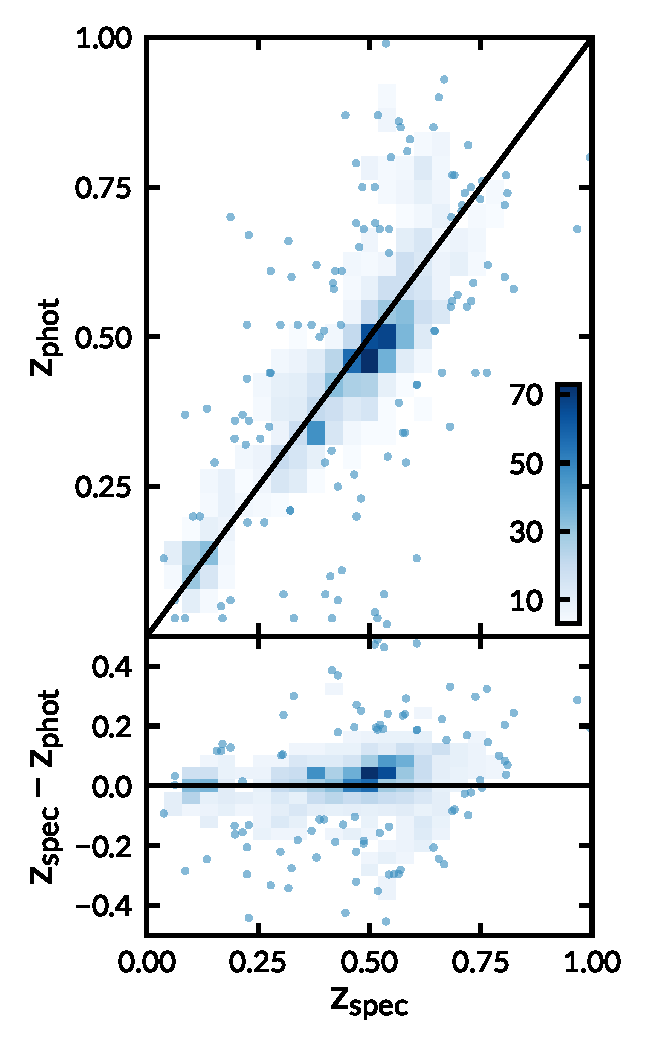
\includegraphics[width=\columnwidth]{figures/specVSphot.pdf}
	\caption{Comparison between photometric and spectroscopic redshifts for 2253 galaxies which have spectroscopic redshifts from the SDSS. The photometric redshifts in the top panel use a Bayesian approach with a custom empirical prior on galaxy brightness for the photometric redshifts. The bottom panel shows the difference between the spectroscopic and photometric redshift.}
	\label{fig:photozspecz}
\end{figure}

Figure~\ref{fig:photozspecz} shows the photometric redshift performance as a function of the true spectroscopic redshift. For the full sample of galaxies we calculate $\sigma_f = \editorial{XX\%}$, $\sigma_{NMAD} = \editorial{XX\%}$, and an outlier fraction, $\eta = \editorial{XX\%}$. When considering the performance of only the galaxies BPZ classified as E and E/S0 type, we find the following results; $\sigma_f = 10.4\%$, $\sigma_{NMAD} = 5.43\%$, and an outlier fraction, $\eta = 2.97\%$.

\subsection{Cluster Finding}
In this section, we briefly describe the algorithms and methods use to select the galaxy clusters from the multi-wavelength optical imaging. We follow the methods described in detail in \cite{Menanteau2009a, Menanteau2010}. We direct the reader there for an in depth description and discussion of the methods.

We first create a three-color image using \textsc{stiff} \citep{Bertin2011}. The red, green, and blue channels are given by the corresponding combined mosaics described in Section~\ref{sec:mosaicks}. We then visually inspect an area of roughly $8' \times 8'$ centered on the position of each unconfirmed cluster; see Table~\ref{tbl:targets}. Potential brightest cluster galaxies (BCGs) are identified by first calculating the absolute limiting magnitude \editorial{needs details}.

Once a potential BCG is selected, the algorithm selects nearby galaxies, within $|z_{BCG} - z| < 0.05$ and 0.5 Mpc projected radius, which BPZ has classified as either E or E/S0 galaxies. These photo-z's of the galaxies are combined using a $3\sigma$ median sigma-clipping algorithm to estimate the cluster's mean redshift, $z_c$. We use this mean cluster redshift measurement and the member selection criteria given previously to estimate the number of cluster members within 1 Mpc, $N_{1\rm Mpc}$, which we define as the richness of the cluster, $N_{gal}$.

We correct the $N_{gal}$ estimate by subtracting a statistical background of galaxies. We first estimate the number of background ellipticals by selecting galaxies within an annulus ($R_{200} <r < 2R_{200}$) around each cluster's position. We include galaxies with $\delta z = 0.05$ and similar colors as those galaxies assumed to belong to the cluster. These galaxies are subtracted from the cluster's population which provides an corrected $N_{gal}$, $N_{galc}$, which we then use to compute other important quantities. In practice the corrected number of galaxies is between 15\% and 20\% lower than the uncorrected number \citep{Menanteau2010}. We report $N_{galc}$ for the remainder of this work.

\subsection{Recovery of the Brightest Cluster Galaxies}
We have designed our observations to detect BCGs to $z\sim1.5$. To quantify the actual depth of our images, we perform a Monte Carlo simulation by injecting artificial sources and computing their recovery fraction. We create the artificial sources with the \textsc{modeling} package, part of \textsc{astropy} \citep{TheAstropyCollaboration2013}.

Following the procedure given in \cite{Menanteau2010a}, the synthetic galaxies are created to have de Vaucouleurs \citep{DeVaucouleurs1948} profiles and surface brightnesses corresponding to their magnitude and assumed sizes. We inject the artificial galaxies into our science images with similar noise characteristics as their real counterparts.

We generate four rounds of one hundred elliptical galaxies spread uniformly across our science imaging. Each round of galaxies are place at different random positions to suppress abnormally boosted recovery fractions due to source confusion. The artificial galaxies have total fluxes corresponding to apparent magnitudes between 19 mag $< \sdssi <$ 27 mag with 0.1 mag spacing.

\begin{figure*}
	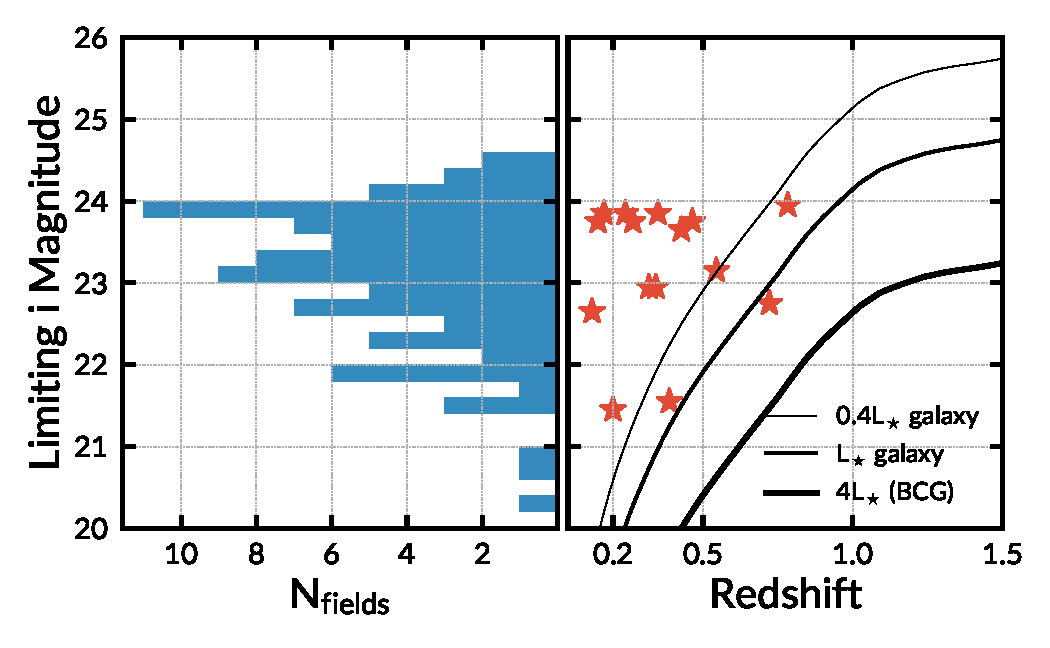
\includegraphics[width=\textwidth]{figures/recovery_redshift.pdf}
	\caption{\textit{Left:} Histogram of the \sdssi-band magnitude corresponding to 80\% completeness in galaxy recovery. When 80\% completeness is not achieved we show the limiting magnitude with the highest completeness. \textit{Right:} Observed \sdssi-band magnitudes of L$_{\star}$, 0.4L$_{\star}$, and 4L$_{\star}$ (BCG) early-type galaxies as a function of redshift. We define an L$_{\star}$ galaxy following \cite{Blanton2003} as a population of red galaxies at $z = 0.1$ and allow it to evolve passively. The left and right panels can be combined to estimate the limiting redshift to which we could identify galaxy clusters.}
	\label{fig:recovery_redshift}
\end{figure*}

\editorial{This is almost directly taken from FM2010 -- edit.} We use the individual field's completion limit to estimate the redshift to which we can reliably detect massive clusters. For this, we compare the completeness limits of our observations to the expected and observed (\ie, known) apparent magnitudes of galaxies in clusters as a function of redshift. We estimated the expected apparent galaxy \sdssi-band magnitude as a function of redshift using L$_{\star}$ as defined for the population of red galaxies by \cite{Blanton2003} at $z = 0.1$ and allowing passive evolution according to a solar metallicity \citep{Bruzual2003} $\tau = 1.0$ Gyr burst model formed at $zf = 5$. We show this in Figure~\ref{fig:recovery_redshift} for a range of luminosities (L$_{\star}$, 0.4L$_{\star}$, and 4L$_{\star}$) aimed at representing the cluster members from the faint ones to the BCG.

\section{Results}\label{sec:results}

\begin{table*}
	\caption[Caption]{Caption}

	\tiny
\begin{tabular}{lllrrrrrllrrlr}
	\hline
	Name &    RA PSZ &       DEC PSZ &  RA &  DEC &  Dist &    z &  Mag Lim &         RA EX &        DEC EX &  Dist EX &  z EX & Flag &   Ref \\
	\hline
 PSZ1\_G031.91+67.94 &  14:29:02 &  +24:37:33.38 & NaN &  NaN &   NaN & 0.70 &    23.20 &  14:30:23.299 &  +24:39:06.19 &    18.54 &  0.13 &  NaN &  50.0 \\
 PSZ1\_G055.83-41.64 &  21:57:14 &      -2:31:51 & NaN &  NaN &   NaN & NaN &    23.44 &   21:56:41.02 &  -02:32:20.87 &     8.25 &  0.63 &    3 &  -1.0 \\
 PSZ1\_G084.62-15.86 &  21:49:44 &  +33:10:23.81 & NaN &  NaN &   NaN & 0.30 &    22.93 &  21:49:40.599 &  +33:10:34.59 &     0.73 &  0.37 &  NaN &  50.0 \\
 PSZ1\_G096.44-10.40 &  22:19:35 &  +44:31:05.27 & NaN &  NaN &   NaN & NaN &    22.80 &   22:20:12.95 &  +44:26:16.27 &     8.31 &  0.20 &   ND &  -1.0 \\
 PSZ1\_G102.86-31.07 &  23:33:08 &  +28:43:51.60 & NaN &  NaN &   NaN & 0.49 &    23.58 &  23:33:24.699 &  +28:43:19.89 &     3.70 &  0.59 &  NaN &  50.0 \\
 PSZ1\_G102.97-04.77 &  22:34:47 &  +52:43:13.90 & NaN &  NaN &   NaN & NaN &    21.56 &   22:34:47.08 &  +52:42:55.56 &     0.31 &  0.52 &    2 &  -1.0 \\
 PSZ1\_G108.90-52.04 &   0:16:38 &  +09:52:49.98 & NaN &  NaN &   NaN &  NaN &    23.48 &   00:16:26.74 &  +09:53:53.60 &     2.97 &  0.46 &    2 &  -1.0 \\
 PSZ1\_G118.06+31.10 &  15:54:34 &  +84:10:37.49 & NaN &  NaN &   NaN & 0.41 &    22.69 &  15:54:38.699 &  +84:10:28.39 &     0.19 &  0.19 &  NaN &  50.0 \\
 PSZ1\_G138.60-10.85 &   2:27:02 &  +49:04:54.07 & NaN &  NaN &   NaN & 0.64 &    23.43 &  02:27:06.699 &  +49:00:29.29 &     4.48 &  0.70 &  NaN &  50.0 \\
 PSZ1\_G142.17+37.28 &   9:18:56 &  +70:52:01.14 & NaN &  NaN &   NaN & 0.24 &    23.30 &   09:19:05.16 &  +70:55:11.40 &     3.26 &  0.28 &    1 &  10.0 \\
 PSZ1\_G142.38+22.82 &   6:13:40 &  +71:52:21.02 & NaN &  NaN &   NaN & NaN &    22.95 &   06:13:49.84 &  +71:52:54.78 &     0.95 &  0.39 &    2 &  -1.0 \\
 PSZ1\_G146.00-49.42 &   1:51:35 &  +10:44:02.79 & NaN &  NaN &   NaN & NaN &    23.56 &  01:51:19.799 &  +10:47:29.99 &     5.09 &  0.10 &  NaN &  50.0 \\
 PSZ1\_G148.20+23.49 &   6:37:46 &  +66:54:24.40 & NaN &  NaN &   NaN &  NaN &    23.21 &   06:37:54.60 &  +66:51:06.20 &     3.41 &  0.11 &    2 &  10.0 \\
 PSZ1\_G153.41+36.58 &   8:42:40 &  +62:34:31.61 & NaN &  NaN &   NaN & 0.64 &    23.35 &  08:42:42.899 &  +62:30:21.59 &     4.18 &  0.65 &  NaN &  50.0 \\
 PSZ1\_G153.56+36.23 &   8:39:31 &  +62:31:30.58 & NaN &  NaN &   NaN & 0.31 &    23.27 &  08:39:33.399 &  +62:26:12.09 &     5.32 &  0.13 &  NaN &  50.0 \\
 PSZ1\_G162.30-26.92 &   3:24:26 &  +24:00:44.46 & NaN &  NaN &   NaN & NaN &    23.32 &   03:24:19.02 &  +23:57:49.82 &     3.32 &  0.39 &    2 &  -1.0 \\
 PSZ1\_G169.80+26.10 &   7:30:08 &  +48:20:02.06 & NaN &  NaN &   NaN & 0.62 &    23.35 &   07:30:32.02 &  +48:17:39.05 &     4.65 &  0.73 &    2 &  -1.0 \\
 PSZ1\_G183.26+12.25 &   6:42:56 &  +31:49:07.58 & NaN &  NaN &   NaN & NaN &    20.77 &   06:43:09.84 &  +31:50:55.47 &     3.45 &  0.85 &    2 & 500.0 \\
 PSZ1\_G185.93-31.21 &   4:11:39 &  +06:16:00.67 & NaN &  NaN &   NaN & NaN &    22.71 &   04:11:52.31 &  +06:17:11.80 &     3.51 &  0.09 &    2 &  -1.0 \\
 PSZ1\_G206.45+13.89 &   7:29:59 &  +11:56:22.64 & NaN &  NaN &   NaN & 0.41 &    20.00 &   07:29:51.23 &  +11:56:30.89 &     1.91 &  0.38 &    1 &  10.0 \\
 PSZ1\_G224.82+13.62 &   8:01:42 &      -4:03:54 & NaN &  NaN &   NaN & 0.16 &    22.91 &   08:01:41.61 &  -04:03:46.23 &     0.16 &  0.29 &    1 &  10.0 \\
 PSZ1\_G249.01+73.75 &  11:56:46 &  +16:55:43.68 & NaN &  NaN &   NaN & NaN &    23.08 &  11:57:05.599 &  +16:57:35.39 &     5.04 &  0.16 &  NaN &  50.0 \\
 PSZ1\_G286.25+62.68 &  12:21:10 &  +00:47:34.05 & NaN &  NaN &   NaN & 0.46 &    23.35 &   12:21:05.35 &  +00:48:22.29 &     1.41 &  0.21 &    3 &  -1.0 \\
 PSZ1\_G341.69+50.66 &  14:25:20 &      -4:59:54 & NaN &  NaN &   NaN & 0.28 &    22.25 &   14:25:12.29 &  -04:56:34.19 &     3.84 &  0.30 &    1 &  10.0 \\
 PSZ2\_G022.03+17.75 &  17:28:37 &      -1:13:03 & NaN &  NaN &   NaN & 0.27 &    23.17 &   17:28:16.01 &  -01:22:58.04 &    11.22 &  0.65 &    1 &  -1.0 \\
 PSZ2\_G032.12-14.96 &  19:43:34 &      -7:27:45 & NaN &  NaN &   NaN & NaN &    22.51 &   19:43:11.20 &  -07:24:56.25 &     6.31 &  0.38 &    3 &  -1.0 \\
 PSZ2\_G033.27-17.54 &  19:54:52 &      -7:36:11 & NaN &  NaN &   NaN & NaN &    22.64 &   19:54:59.67 &  -07:30:34.70 &     5.92 &  0.33 &    2 &  -1.0 \\
 PSZ2\_G071.67-42.76 &  22:30:54 &  +05:42:05.22 & NaN &  NaN &   NaN & 0.73 &    23.56 &   22:30:50.00 &  +05:39:16.72 &     2.98 &  0.69 &   ND &  -1.0 \\
 PSZ2\_G093.04-32.38 &  23:01:43 &  +24:02:24.90 & NaN &  NaN &   NaN & NaN &    22.46 &   23:02:15.07 &  +24:03:50.50 &     7.46 &  0.51 &    3 &  -1.0 \\
 PSZ2\_G310.81+83.91 &  12:55:01 &  +21:05:41.16 & NaN &  NaN &   NaN & NaN &    21.23 &           NaN &           NaN &      NaN &  0.45 &  NaN &   2.0 \\
	\hline
\end{tabular}
\label{tbl:preobserved}
\end{table*}

In this section we give the results of our visual cluster finding. During the inspection of each field, we classify each into four possible catalogs: High confidence, medium confidence, low confidence, and no detection. A high confidence result consists of a clear BCG and many accompanying satellite galaxies (see Figure~\ref{fig:high confidence}). A low confidence result is an ambiguous system where there is no clear BCG present but there appears to be a grouping of galaxies at a similar redshift. The medium confidence results fall in between the high and low confidence regimes where there appears to be a BCG but few satellite galaxies are observed. We fail to observe a cluster when there is no clear BCG candidate or clear group of galaxies at similar redshifts.

For the \editorial{112 fields} observed with MOSAIC, we observe \editorial{twelve} high confidence clusters, twenty two both medium and low confidence clusters, and we observe no discernible cluster in sixty fields. In the following subsections we present on each of the eight high confidence observations individually, and group the medium and low confidence observations together.

\subsection{Observations of Known Clusters}

During the course of our observation campaign thirty clusters were confirmed through either dedicated follow up from the \textit{Planck} team (\eg, \citealt{PlanckCollaboration2015, PlanckCollaboration2016a}) or through independent programs (\eg, \citealt{Liu2015a, VanderBurg2016, Burenin2017, Burenin2018, Amodeo2018, Barrena2018, Streblyanska2018}). We can use this opportunity to validate our cluster detection method against known clusters. The thirty clusters are indicated in Table~\ref{tbl:preobserved}.

We successfully recovery \editorial{ten} clusters. For the previously confirmed clusters which we cannot independently confirm, we discuss the potential reasons below.

\subsubsection{PSZ1 G031.91+67.94}

The position of the cluster reported in \cite{PlanckCollaboration2016a} is $\sim18\farcm5$ from the reported PSZ1 position. We do not confirm a cluster within the $5'$ search radius used in our study.

\subsubsection{PSZ1 G084.62-15.86}
We recover a cluster at $z_{cl} = 0.271 \pm 0.099$ with 18 members. This is a system with at least three possible BCGs.

\subsubsection{PSZ1 G102.86-31.07}
We recover a cluster at $z_{cl} = 0.497 \pm 0.136$ with 13 possible members.

\subsubsection{PSZ1 G102.97-04.77}
Low galactic latitude make recovering any previously known cluster very difficult.

\subsubsection{PSZ1 G183.26+12.25}
Due to poor observing conditions, this field has a significantly lower limiting redshift \editorial{give number}. We are unable to confirm this cluster with $z=0.85.$

\subsubsection{PSZ1 G206.45+13.89}
We find a cluster at $z_{cl} = 0.399 \pm 0.05$. We detect 73 potential cluster members, although a bright star (V $= 4.5$ mag; \citealt{Hog2000}) only $\sim4\farcm9$ away from the reported BCG. The contaminating star prevents an accurate photo-z estimate for many cluster cluster members.

\subsubsection{PSZ1$\_$G224.82+13.62}
previously confirmed

\subsubsection{PSZ2 G022.03+17.75}

\textit{PSZ2 G022.03+17.75} is previously reported as \textit{PSZ1 G021.88+17.75} in \cite{PlanckCollaboration2014}. The position in the PSZ1 catalog differs signifcantly, \editorial{give numbers} from the position in the PSZ2 catalog. The position reported by \cite{Barrena2018} corresponds to the PSZ1 position. Because our study assumes the PSZ2 catalog replaces the corresponding entries in PSZ1 catalog, we cannot confirm a cluster within the search radius around the PSZ2 position.

\subsubsection{PSZ2 G033.27-17.54}
\editorial{it looks like this BCG falls into the chipgap due to the observation strategy. I don't think we found this cluster because the BCG wasn't observed.}


\subsection{Newly Discovered Clusters}

%\begin{figure*}
%	\begin{center}
%		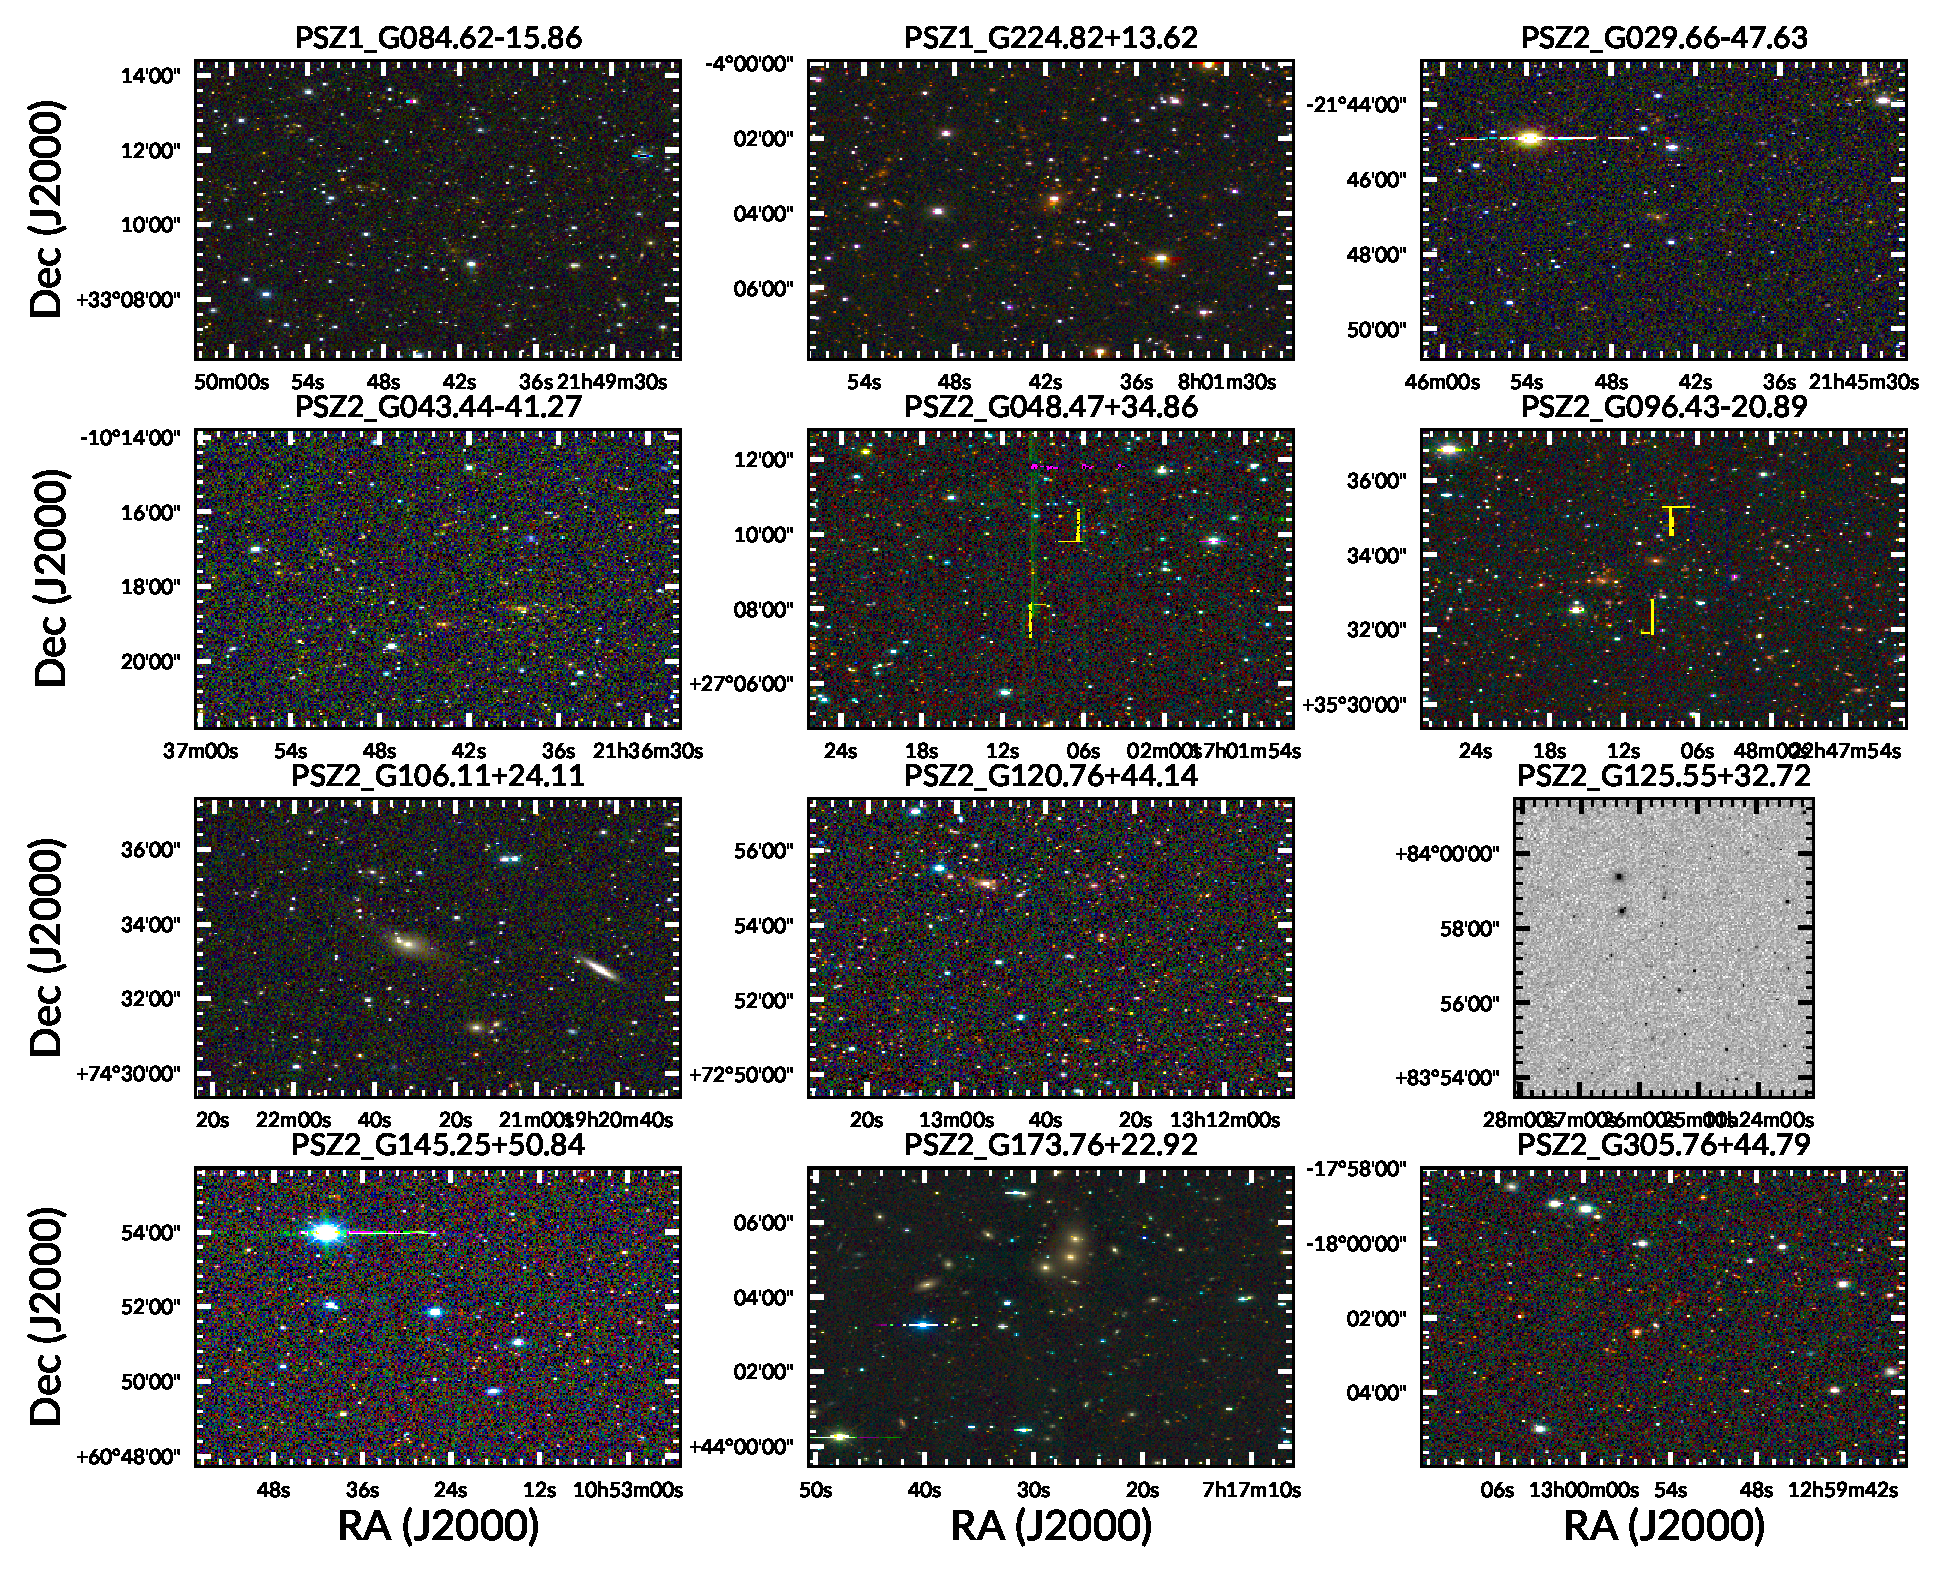
\includegraphics[width=\textwidth]{./figures/result_mosaic.pdf}
%	\end{center}
%	\caption[Montage of remaining nine clusters]{This is a placeholder figure for our high confidence clusters. I'm planning on making something similar.}
%	\label{fig:high confidence}
%\end{figure*}

Lorem ipsum dolor amet swag copper mug meh tilde, put a bird on it live-edge tattooed kinfolk before they sold out locavore selvage leggings raclette literally bicycle rights. Hot chicken kickstarter mustache vinyl roof party. Wayfarers brooklyn truffaut twee umami, venmo irony. Typewriter viral pop-up, listicle vaporware organic af salvia keytar twee chillwave austin +1 offal blog. La croix dreamcatcher snackwave, try-hard intelligentsia taxidermy messenger bag air plant godard mustache celiac glossier echo park. Photo booth readymade authentic glossier biodiesel snackwave beard hammock sriracha before they sold out edison bulb fixie PBR\&B. Man bun pabst kogi, crucifix subway tile af tacos cray tumeric lyft cronut lomo tattooed.


\subsubsection{PSZ2 G029.66-47.63}

\subsubsection{PSZ2 G043.44-41.27}

\subsubsection{PSZ2 G096.43-20.89}

\subsubsection{PSZ2 G125.55+32.72}

\subsubsection{PSZ2 G173.76+22.92}

\subsubsection{PSZ2 G305.76+44.79}

\subsection{Redshift Limits in Other Fields}

Lorem ipsum dolor amet swag copper mug meh tilde, put a bird on it live-edge tattooed kinfolk before they sold out locavore selvage leggings raclette literally bicycle rights. Hot chicken kickstarter mustache vinyl roof party. Wayfarers brooklyn truffaut twee umami, venmo irony. Typewriter viral pop-up, listicle vaporware organic af salvia keytar twee chillwave austin +1 offal blog. La croix dreamcatcher snackwave, try-hard intelligentsia taxidermy messenger bag air plant godard mustache celiac glossier echo park. Photo booth readymade authentic glossier biodiesel snackwave beard hammock sriracha before they sold out edison bulb fixie PBR\&B. Man bun pabst kogi, crucifix subway tile af tacos cray tumeric lyft cronut lomo tattooed.

\section{Discussion}\label{sec:discussion}

Lorem ipsum dolor amet swag copper mug meh tilde, put a bird on it live-edge tattooed kinfolk before they sold out locavore selvage leggings raclette literally bicycle rights. Hot chicken kickstarter mustache vinyl roof party. Wayfarers brooklyn truffaut twee umami, venmo irony. Typewriter viral pop-up, listicle vaporware organic af salvia keytar twee chillwave austin +1 offal blog. La croix dreamcatcher snackwave, try-hard intelligentsia taxidermy messenger bag air plant godard mustache celiac glossier echo park. Photo booth readymade authentic glossier biodiesel snackwave beard hammock sriracha before they sold out edison bulb fixie PBR\&B. Man bun pabst kogi, crucifix subway tile af tacos cray tumeric lyft cronut lomo tattooed.

\section{Summary}\label{sec:summary}

Lorem ipsum dolor amet swag copper mug meh tilde, put a bird on it live-edge tattooed kinfolk before they sold out locavore selvage leggings raclette literally bicycle rights. Hot chicken kickstarter mustache vinyl roof party. Wayfarers brooklyn truffaut twee umami, venmo irony. Typewriter viral pop-up, listicle vaporware organic af salvia keytar twee chillwave austin +1 offal blog. La croix dreamcatcher snackwave, try-hard intelligentsia taxidermy messenger bag air plant godard mustache celiac glossier echo park. Photo booth readymade authentic glossier biodiesel snackwave beard hammock sriracha before they sold out edison bulb fixie PBR\&B. Man bun pabst kogi, crucifix subway tile af tacos cray tumeric lyft cronut lomo tattooed.

\section*{Acknowledgements}
This research made use of several open source packages: \textsc{APLpy}, an open-source plotting package for Python hosted at \url{http://aplpy.github.com}; the \textsc{IPython} package \citep{Perez2007}; \textsc{matplotlib}, a Python library for publication quality graphics \citep{Hunter2007} and \textsc{Astropy}, a community developed core Python package for Astronomy \citep{TheAstropyCollaboration2013}.
\textsc{iraf} is distributed by the National Optical Astronomy Observatory, which is operated by the Association of Universities for Research in Astronomy under cooperative agreement with the National Science Foundation \citep{Tody1993}.
\textsc{PyRAF} is a product of the Space Telescope Science Institute, which is operated by AURA for NASA.
Funding for the SDSS and SDSS-II has been provided by the Alfred P. Sloan Foundation, the Participating Institutions, the National Science Foundation, the U.S. Department of Energy, the National Aeronautics and Space Administration, the Japanese Monbukagakusho, the Max Planck Society, and the Higher Education Funding Council for England. The SDSS Web Site is \url{http://www.sdss.org/}. The SDSS is managed by the Astrophysical Research Consortium for the Participating Institutions.
This work has made use of data from the European Space Agency (ESA) mission {\it Gaia} (\url{https://www.cosmos.esa.int/gaia}), processed by the {\it Gaia} Data Processing and Analysis Consortium (DPAC, \url{https://www.cosmos.esa.int/web/gaia/dpac/consortium}). Funding for the DPAC has been provided by national institutions, in particular the institutions participating in the {\it Gaia} Multilateral Agreement.
This research has made use of the VizieR catalogue access tool, CDS, Strasbourg, France. The original description of the VizieR service was published in \cite{Ochsenbein2000}.
This research has made use of the SVO Filter Profile Service (\url{http://svo2.cab.inta-csic.es/theory/fps/}) supported from the Spanish MINECO through grant AyA2014-55216.

%%%%%%%%%%%%%%%%%%%% REFERENCES %%%%%%%%%%%%%%%%%%
% The best way to enter references is to use BibTeX:
\bibliographystyle{apj}
\bibliography{master}

% if your bibtex file is called example.bib
%%%%%%%%%%%%%%%%% APPENDICES %%%%%%%%%%%%%%%%%%%%%

\end{document}
